%%
%% VERSION HISTORY
%%    22 May 2006 - John Papandriopoulos - Original version
%%    12 Jul 2007 - John Papandriopoulos - Converted into template
%%

\documentclass[11pt,a4paper,titlepage,twoside,openright]{book}

% Use the UniMelb Dissertation Template
\usepackage{style/uomthesis}

% User defined commands
%%
%% VERSION HISTORY
%%    22 May 2006 - John Papandriopoulos - Original version
%%    12 Jul 2007 - John Papandriopoulos - Converted into template
%%    30 Sep 2015 - Maoyuan Liu - Draft version
%%

%%
%% Custom Hyphenations
%%

\hyphenation{cross-talk}

%%
%% Sample custom-configuration
%%
%%   You are encouraged to modify the following section with any of your
%%   own custom commands, packages, etc.
%%

% for URLs
\usepackage{url}

\usepackage[linktoc=all]{hyperref}
\hypersetup{
    colorlinks,
    citecolor=black,
    filecolor=black,
    linkcolor=black,
    urlcolor=black
}

% AMS packages
%\usepackage{amsfonts}
\usepackage{amssymb}
\usepackage{amsmath}
\usepackage{amsthm}
\usepackage[mathscr]{eucal}

% Allow equations to break over pages...
\interdisplaylinepenalty=2500
% Command to stop equation breaks
% Note: enclose this in braces when used...
\newcommand{\donotsplitoverpages}{\interdisplaylinepenalty=10000}

% Graphics
%\ifx\pdftexversion\undefined
%  \usepackage[dvips]{graphicx}
%\else
%  \usepackage[pdftex]{graphicx}
%\fi
\usepackage{graphicx}

% set page margins
\newcommand{\setoddmargin}[1]{\oddsidemargin \paperwidth
  \addtolength{\oddsidemargin}{-\textwidth}
  \addtolength{\oddsidemargin}{-#1}
  \addtolength{\oddsidemargin}{-1in}}
\newcommand{\setevenmargin}[1]{\evensidemargin \paperwidth
  \addtolength{\evensidemargin}{-\textwidth}
  \addtolength{\evensidemargin}{-#1}
  \addtolength{\evensidemargin}{-1in}}

% Enable IEEE macros
\usepackage{IEEEtrantools}
\newcommand{\PARstart}[2]{\IEEEPARstart{#1}{#2}}

% Use a plain bibliography style
%\bibliographystyle{plain}
% Use the IEEE bibliography style (sorted)
\bibliographystyle{IEEEtrans}
% Use the IEEE bibliography style (unsorted; order of reference)
%\bibliographystyle{IEEEtran}

% For isolated bibliographies
\usepackage{bibunits}

\usepackage{color}
\usepackage{xcolor}
\usepackage[noadjust]{cite}
\usepackage{caption}

% For cool tables
\usepackage{array}

% For subfigures
\usepackage{subfig}
%\usepackage{subfigure}

% For algorithms
\usepackage{algorithm}
\usepackage{algorithmic}

% For cases
\usepackage{sublabel}

% For theroem numbers having the chapter included
\usepackage{style/chngcntr}

% For testing the formatting
\usepackage{lipsum}

% For cool theorem styles
%\usepackage[amsthm]{ntheorem}
%\theorembodyfont{\normalfont}

% Theorem definition
\newtheorem{theorem}{Theorem}
\counterwithin{theorem}{chapter}

% Corollary definition
\newtheorem{corollary}{Corollary}
\counterwithin{corollary}{chapter}

% Result definition
\newtheorem{result}{Result}
\counterwithin{result}{chapter}

% Lemma definition
\newtheorem{lemma}{Lemma}
\counterwithin{lemma}{chapter}

% Proposition definition
\newtheorem{proposition}{Proposition}
\counterwithin{proposition}{chapter}

% Definition definition!
\newtheorem{definition}{Definition}
\counterwithin{definition}{chapter}

% Remark definition (no counter?)
\newenvironment{remark}{\emph{Remark:~}}{}

% Fact definition (no counter?)
\newenvironment{fact}{\emph{Fact:~}}{}

% (Re)Set the figure path
\newcommand{\setfigurepath}[1]{%
\ifx\figurepath\undefined
	\newcommand{\figurepath}{#1}
\else
	\renewcommand{\figurepath}{#1}
\fi%
}

% Used in the continued list environment below
\newcounter{continuedlist}

% Continued list environment
\newenvironment{continuedlist}{%
	\begin{enumerate}%
		% Space out each item
		\setlength{\itemsep}{1.25em}%
		% Start the enumeration from the previous value
		\setcounter{enumi}{\value{continuedlist}} 
}{%
		% Save the counter to continue it later
		\setcounter{continuedlist}{\value{enumi}}%
	\end{enumerate}%
	%\vspace{1.25em}%
	\vspace{1em}%
}

% Spaced out list environment
\newenvironment{spacedoutlist}{%
	\begin{itemize}%
		% Space out each item
		\setlength{\itemsep}{1.25em}%
}{%
	\end{itemize}%
}

% Suppress "This page intentionally left blank."
\newcommand{\markblankpages}{}

% Commands for printing draft
\usepackage{background}
\usepackage[yyyymmdd,hhmmss]{datetime}
\newcommand\DraftText{Draft compiled on \today\ at \currenttime}
\newcommand{\draft}{
  \setoddmargin{3cm}
  \setevenmargin{3cm}
  \backgroundsetup{
    color=lightgray,
    position=current page.center,
    angle=90,
    vshift=0.45\paperwidth,
    opacity=1,
    scale=1,
    contents={\LARGE\ttfamily\DraftText}
  }
}


% suppress "Produced on archival quality paper." on the title page
\newcommand{\archivalpapernote}{}

% set draft watermark
\draft

% set margins to be even
%\setoddmargin{3cm}
%\setevenmargin{3cm}

\begin{document}

	%%
	%% Front matter
	%%
	\begin{frontmatter}

		\frontmatterheadings

		% Collect the dissertation information for the title page
		% Dissertation title
\title{Working Title}

% Author
\author{Maoyuan Liu}

% Date of submission
\submissionmonth{January}
\submissionyear{2016}

% Department
\department{School of Chemistry}

% University
\university{\scshape The University of Melbourne}

		% Generate the title page
		\maketitle

		\begin{abstract}%

{\scshape A long time ago in a galaxy far far away...}

It is a period of civil war. Rebel spaceships, striking from a hidden base, have won their first victory against the evil Galactic Empire.

During the battle, rebel spies managed to steal secret plans to the Empire's ultimate weapon, the DEATH STAR, an armored space station with enough power to destroy an entire planet.

Pursued by the Empire's sinister agents, Princess Leia races home aboard her starship, custodian of the stolen plans that can save her people and restore freedom to the galaxy....

\end{abstract}


		% Author declaration
		\makedeclaration

		% Acknowledgements
		\begin{acknowledgements}
    I would like to thank Han Solo who ran the fastest parsec the likes of which the world has never seen the likes of which.
\end{acknowledgements}


		% Preface
		%%%
%% VERSION HISTORY
%%    22 May 2006 - John Papandriopoulos - Original version
%%    12 Jul 2007 - John Papandriopoulos - Converted into template
%%

% Optional preface to the dissertation
\begin{preface}

	An optional preface is found in the \texttt{preface.tex} file.

\end{preface}



		% Dedications...
		\begin{dedication}
	To my templator, John Papandriopoulos.
\end{dedication}


		% TOC, LOF, LOT
		{%
			\singlespacing%
			\tableofcontents%
			\listoffigures%
			% Do not include a list of tables if you have less
			% than 10 tables, as per SGS suggestion.
			\listoftables%
		   \clearpage%
		}%

   \end{frontmatter}

	%%
	%% Main matter
	%%
	\begin{mainmatter}

		\mainmatterheadings

		% path to figures directory
\graphicspath{{figures/chapter-1/}}

%=========================================================================

\begin{savequote}[75mm]
Nulla facilisi. In vel sem. Morbi id urna in diam dignissim feugiat. Proin molestie tortor eu velit. Aliquam erat volutpat. Nullam    ultrices, diam tempus vulputate egestas, eros pede varius leo.
\qauthor{Quoteauthor Lastname}
\end{savequote}

\chapter{Introduction}
	\label{chapter:introduction}
	%

%=========================================================================

\section{Introduction}

\lipsum[1-6]\cite{Mao}
\index{a}
\myglossaryentry{lipsum}{lipsum}{Lorem Ipsum, a special type of fudge}{}
\myglossaryentry{dolor}{dolor}{No idea why}{parent={lipsum}}
\myglossaryentry{ibit}{ibit}{Sounds right, doesn't it?}{parent={lipsum}}
\myacronym{DFT}{density functional theory}
%\myglossaryentry{\ensuremath{\pi}}{pi}{Greek letter pi, \ensuremath{\Pi} does this work?}{symbol={\ensuremath{\pi}}, sort=pi}
\myglossaryentry{$\pi$}{pi}{Greek letter pi, \ensuremath{\Pi} does this work?}{symbol={$\pi$}}
\myacronym{RDF}{radial distribution function}
\myglossaryentry{radial distribution function}{radialdistributionfunction}{}{symbol={$g(r)$}}

\begin{figure}[h]
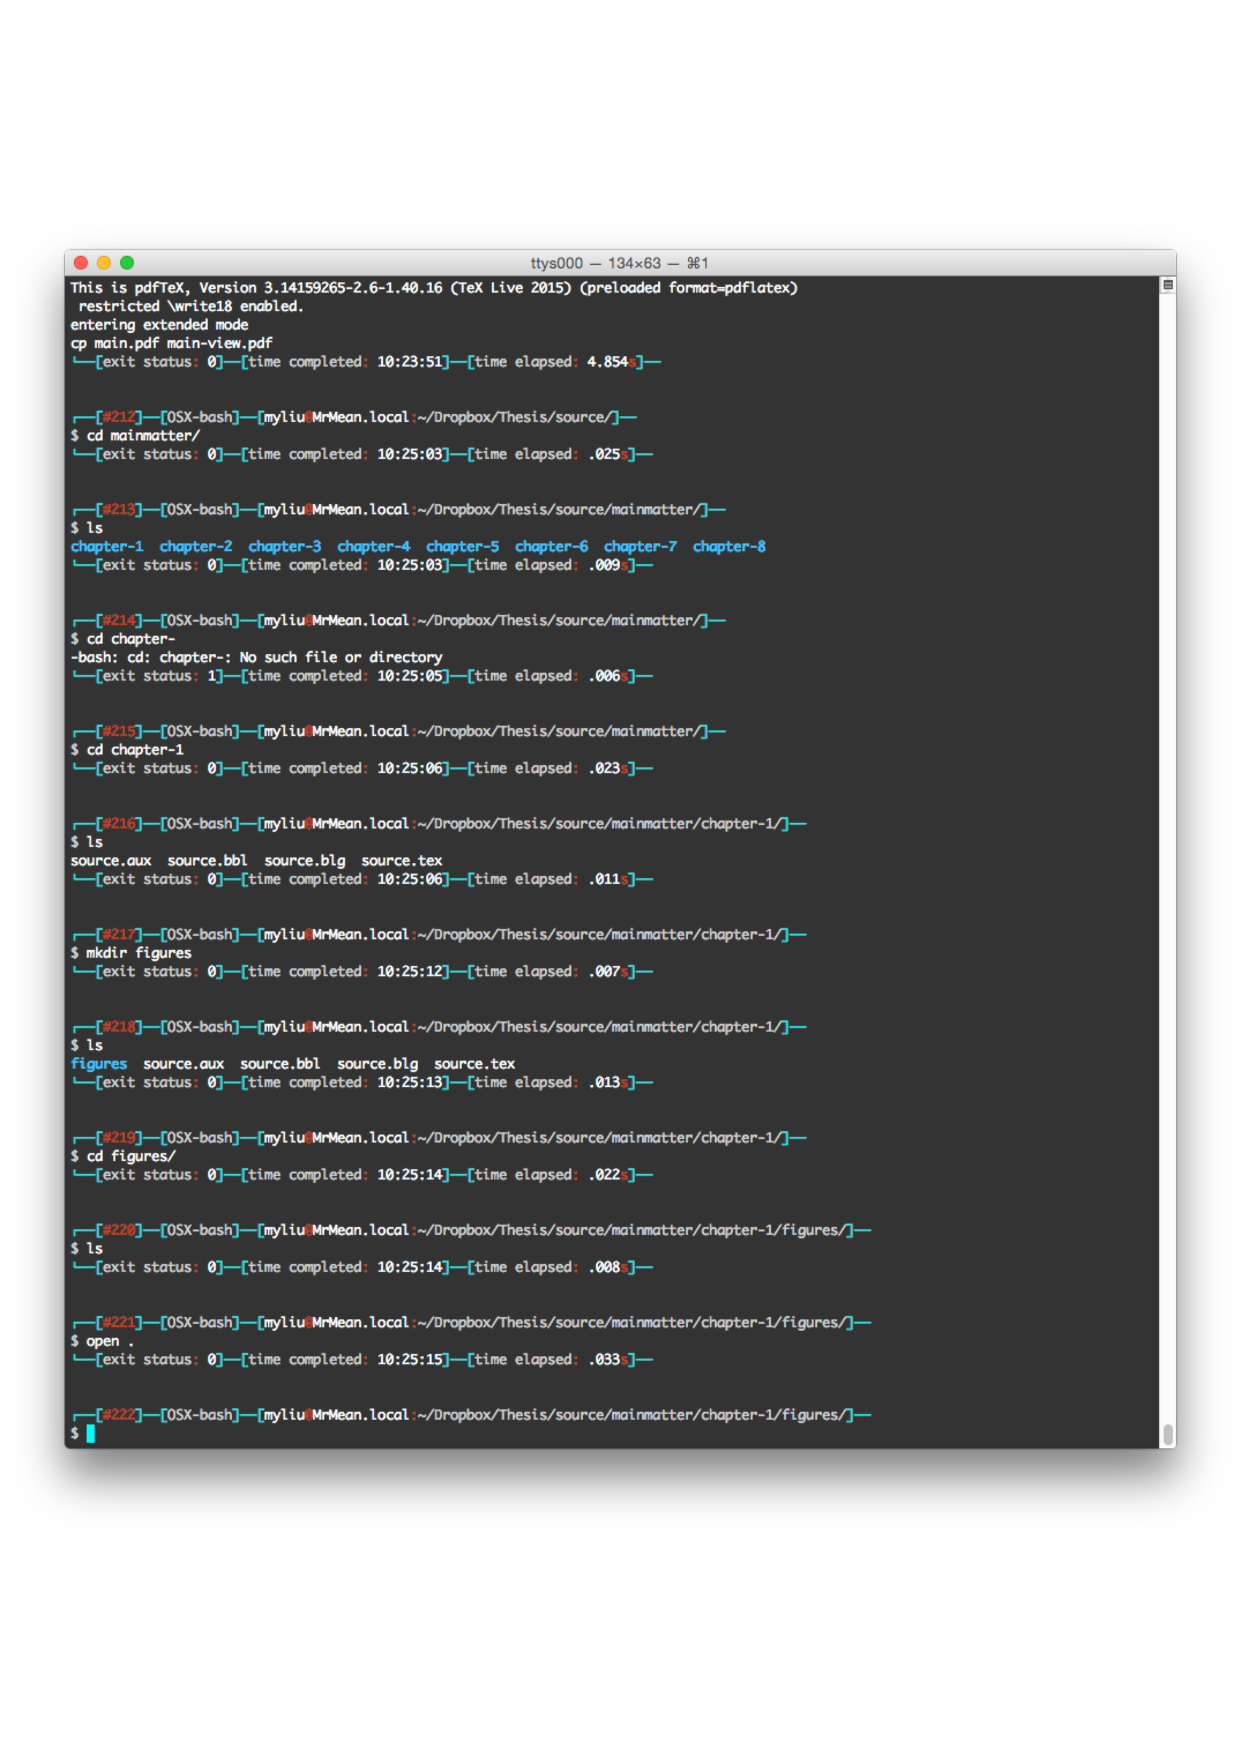
\includegraphics[height=0.7\textheight]{a.pdf}
\caption[This is a short caption]{This is a terminal screen for stuff.\cite{Mao}}
\end{figure}

%=========================================================================

\mybib{bib/test.bib}

    \chapter{The Phantom Menace}
	%\label{chapter:}

% preferred location for figures in this chapter
\graphicspath{{figures/chapter-2/}}

%=========================================================================

\begin{synopsis}
	In this chapter...
\end{synopsis}

%=========================================================================

\section{Introduction}

\lipsum[1-4] \index{amet}
\cite{Lorch1969}

\mybib{bib/test.bib}

    \chapter{The Empire Strikes Back}
	\label{chapter:empire-strikes-back}%
	%

% preferred location for figures in this chapter
\setfigurepath{figures/chapter-3}

%=========================================================================

\begin{synopsis}
	Synopsis.
\end{synopsis}

%=========================================================================

\section{Introduction}

\PARstart{U}{se} the force Luke...\cite{Salmon2006}

\mybib{bib/test.bib}

    % path to figures directory
\graphicspath{{figures/chapter-4/}}

%=========================================================================

\begin{savequote}[75mm]
Nulla facilisi. In vel sem. Morbi id urna in diam dignissim feugiat. Proin molestie tortor eu velit. Aliquam erat volutpat. Nullam    ultrices, diam tempus vulputate egestas, eros pede varius leo.
\qauthor{Quoteauthor Lastname}
\end{savequote}

\chapter{Return of the Sith}
  %\label{chapter:}

%=========================================================================

\section{Introduction}

\lipsum[15-19]
\cite{Salmon2006}

%=========================================================================

\mybib{bib/test.bib}

    \chapter{The Phantom Menace}
	\label{chapter:phantom-menace}%
	%

% preferred location for figures in this chapter
\setfigurepath{figures/chapter-5}

%=========================================================================

\begin{synopsis}
	Synopsis.
\end{synopsis}

%=========================================================================

\section{Introduction}

\PARstart{U}{se} the force Luke...


    % path to figures directory
\graphicspath{{figures/chapter-6/}}

%=========================================================================

\begin{savequote}[75mm]
Nulla facilisi. In vel sem. Morbi id urna in diam dignissim feugiat. Proin molestie tortor eu velit. Aliquam erat volutpat. Nullam    ultrices, diam tempus vulputate egestas, eros pede varius leo.
\qauthor{Quoteauthor Lastname}
\end{savequote}

\chapter{The Empire Strikes Back}
  %\label{chapter:}

%=========================================================================

\section{Introduction}

\lipsum[100]
\cite{Salmon2006}

%=========================================================================

\mybib{bib/test.bib}


	\end{mainmatter}

	%%
	%% Appendix
	%%
	\begin{appendix}

		\chapter{Appendix}
		\label{appendix}

%=========================================================================

\section{The Force Awakens}

\lipsum[50-55]\cite{Drewitt2015}

%=========================================================================
\mybib{bib/test.bib}



	\end{appendix}

	%%
	%% Bibliography
	%%
	\begin{backmatter}

		\chapter*{\bibname}%
		\markboth{\MakeUppercase\bibname}{\MakeUppercase\bibname}%
		%
		% Uncomment the following line to produce a
		% bibliography list of all entries in the bib database
		%\nocite{*}
		%
		\bibliography{%
			% Place your bib database files here, for example:
			%bib/strings,%
			%bib/wireless,%
			%bib/dsl,%
			%bib/selfpubs%
		}
	\end{backmatter}

\end{document}
